% !Mode:: "TeX:UTF-8"
%!TEX program  = xelatex

\documentclass{cumcmthesis}
\usepackage{graphicx}
% \documentclass[withoutpreface,bwprint]{cumcmthesis} %去掉封面与编号页

\usepackage{url}
\title{繁花曲线的分析与绘制}
\tihao{A}
\baominghao{114514}
\schoolname{天元公学}
\membera{陈铭硕}
\memberb{唐铭泽}
\memberc{尹贝尔}
\supervisor{老师}
\date{\today}
\usepackage{footnote}

\usepackage{graphicx}
\usepackage{float}
\usepackage{subfig}

\begin{document}

\maketitle

\begin{abstract}

\keywords{疫情防控\quad  图论\quad   网络流\quad  最短路}
\end{abstract}

%目录
\tableofcontents

\newpage
\section{问题重述}

\subsection{问题的提出}

\section{问题分析}

\subsection{总体分析}

一个居民小区通常由一些单元与道路组成。每个单元都有一定数量的人居住,每条道路都有一定的通过时间。此外,我们可以把道路的交叉点与核酸检测点的候选位置看作没有人
居住的单元。于是我们可以把居民小区抽象为一张无向图,点权为居住人数,边权为边的通过时间,把核酸检测点的规划转化成图论问题进行求解。

\subsection{问题一分析}

定义图上两点的花费为两点的最短路径长度乘上起始点的点权。

建立核酸检测点位置要使居民总体方便,那么建立核酸检测点的位置有两种选择:一种是使得居民到达核酸检测点的总花费最短,另一种是使得到达核酸检测点的最大的花费最
小;并且需要考虑建立的位置是否会给居民的正常生活造成影响。

\subsection{问题二分析}

\subsection{问题三分析}

\section{模型假设}

\section{符号说明}
\begin{center}
\begin{savenotes}
\begin{tabular}{cc}
\hline
\makebox[0.3\textwidth][c]{符号}	&  \makebox[0.4\textwidth][c]{意义} \\ \hline
$n$         & 图的点数 \\ \hline
$m$         & 图的边数 \\ \hline
$w_i$	    & 第 $i$ 个点的点权 \\ \hline
$e_i$	    & 第 $i$ 条边的边权 \\ \hline
$u_i$       & 第 $i$ 条边的起点 \\ \hline
$v_i$       & 第 $i$ 条边的终点 \\ \hline
$d_{i,j}$   & 第 $i$ 个点和第 $j$ 个点最短路径长度 \\ \hline
\end{tabular}
\end{savenotes}
\end{center}

\section{模型建立、求解与分析}

\subsection{问题一}

\subsubsection{选择一}

使得居民到达核酸检测点的总花费最短。

\subsubsection{选择二}

使得到达核酸检测点的最大的花费最小。

提出一个概念叫 \emph{图的绝对重心},定义为到所有点的花费距离的最大值最小的点,那我们的核酸检测点应建立在绝对重心上。

接下来考虑如何求解绝对重心。

\begin{figure}[H]
    \centering
    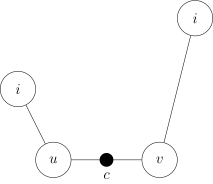
\includegraphics{images/mdst-graph.png}
    \caption{绝对重心求解 1(}
    \label{fig:mdst-graph}
\end{figure}

\subsection{问题二}

我们发现

\section{模型评价}

\newpage

%附录
\begin{appendices}


\end{appendices}

\end{document} 